% A LaTeX (non-official) template for ISAE projects reports
% Copyright (C) 2014 Damien Roque

% This program is free software; you can redistribute it and/or
% modify it under the terms of the GNU General Public License
% as published by the Free Software Foundation; either version 2
% of the License, or (at your option) any later version.

% This program is distributed in the hope that it will be useful,
% but WITHOUT ANY WARRANTY; without even the implied warranty of
% MERCHANTABILITY or FITNESS FOR A PARTICULAR PURPOSE.  See the
% GNU General Public License for more details.

% You should have received a copy of the GNU General Public License
% along with this program; if not, write to the Free Software
% Foundation, Inc., 51 Franklin Street, Fifth Floor, Boston, MA  02110-1301, USA.

% Version: 0.2
% Author: Damien Roque <damien.roque_AT_isae.fr>

\documentclass[openany, a4paper,12pt]{report}
\usepackage[utf8]{inputenc}
\usepackage[T1]{fontenc}
% \usepackage[frenchb]{babel} % If you write in French
\usepackage[english]{babel} % If you write in English
\usepackage{a4wide}
\usepackage{graphicx}
\graphicspath{{images/}}
\usepackage{subfig}
\usepackage{tikz}
\usetikzlibrary{shapes,arrows}
\usepackage{pgfplots}
\pgfplotsset{compat=newest}
\pgfplotsset{plot coordinates/math parser=false}
\newlength\figureheight
\newlength\figurewidth
\pgfkeys{/pgf/number format/.cd,
set decimal separator={,\!},
1000 sep={\,},
}
\usepackage{ifthen}
\usepackage{ifpdf}
\ifpdf
\usepackage[pdftex]{hyperref}
\else
\usepackage{hyperref}
\fi
\usepackage{color}
\hypersetup{%
colorlinks=true,
linkcolor=black,
citecolor=black,
urlcolor=black}

\renewcommand{\baselinestretch}{1.05}
\usepackage{fancyhdr}
\pagestyle{fancy}
\fancyfoot{}
\fancyhead[LE,RO]{\bfseries\thepage}
\fancyhead[RE]{\bfseries\nouppercase{\leftmark}}
\fancyhead[LO]{\bfseries\nouppercase{\rightmark}}
\setlength{\headheight}{15pt}

\let\headruleORIG\headrule
\renewcommand{\headrule}{\color{black} \headruleORIG}
\renewcommand{\headrulewidth}{1.0pt}
\usepackage{colortbl}
\arrayrulecolor{black}

\fancypagestyle{plain}{
  \fancyhead{}
  \fancyfoot[C]{\thepage}
  \renewcommand{\headrulewidth}{0pt}
}

\makeatletter
\def\@textbottom{\vskip \z@ \@plus 1pt}
\let\@texttop\relax
\makeatother

\makeatletter
\def\cleardoublepage{\clearpage\if@twoside \ifodd\c@page\else%
  \hbox{}%
  \thispagestyle{empty}%
  \newpage%
  \if@twocolumn\hbox{}\newpage\fi\fi\fi}
\makeatother

\usepackage{amsthm}
\usepackage{amssymb,amsmath,bbm}
\usepackage{array}
\usepackage{bm}
\usepackage{multirow}
\usepackage[footnote]{acronym}
\usepackage{float}

\usepackage{indentfirst}

% Add Julia code support
\usepackage{listings}
\usepackage{xcolor}

\definecolor{codegreen}{rgb}{0,0.6,0}
\definecolor{codegray}{rgb}{0.5,0.5,0.5}
\definecolor{codepurple}{rgb}{0.58,0,0.82}
\definecolor{backcolour}{rgb}{0.95,0.95,0.92}

\lstdefinelanguage{Julia}%
  {keywords=[1]{abstract,break,case,catch,const,continue,do,else,elseif,%
      end,export,false,for,function,immutable,import,importall,if,in,%
      macro,module,otherwise,quote,return,switch,true,try,type,typealias,%
      using,while,mutable,struct},%
   keywords=[2]{,Int64,Float64,Function,Array,Dict,Network,GridNetwork,NEATIndividual,HyperNEATIndividual,NEATIndiv,Individual,Cambrian,BERLenv,String,GymEnv,}
   sensitive=true,%
   alsoother={$},%
   morecomment=[l]\#,%
   morecomment=[n]{\#=}{=\#},%
   morestring=[s]{"}{"},%
   morestring=[m]{'}{'},%
}[keywords,comments,strings]%

\lstset{%
    language         = Julia,
    basicstyle       = \ttfamily,
    keywordstyle     = [1]\bfseries\color{red},
    keywordstyle     = [2]\bfseries\color{blue},
    backgroundcolor  = \color{backcolour},
    stringstyle      = \color{codepurple},
    commentstyle     = \color{codegray},
    showstringspaces = false,
    breaklines       = true,
    frame            = tblr,
}

% code definition to include code in text
\def\code#1{\texttt{#1}}

\usepackage{url}
%%% display links as blue href 
% \newcommand{\addlink}[2]{\href{#1}{\color{blue}{#2}}}
%%% display links as footnote
\newcommand{\addlink}[2]{\href{#1}{#2}\footnote{\url{#1}}}

\newcommand{\todo}[1]{\textcolor{red}{\MakeUppercase{#1}}}

% Continuous footnotes across whole document
\counterwithout*{footnote}{chapter}

\newcommand*{\SET}[1]  {\ensuremath{\mathbf{#1}}}
\newcommand*{\VEC}[1]  {\ensuremath{\boldsymbol{#1}}}
\newcommand*{\FAM}[1]  {\ensuremath{\boldsymbol{#1}}}
\newcommand*{\MAT}[1]  {\ensuremath{\boldsymbol{#1}}}
\newcommand*{\OP}[1]  {\ensuremath{\mathrm{#1}}}
\newcommand*{\NORM}[1]  {\ensuremath{\left\|#1\right\|}}
\newcommand*{\DPR}[2]  {\ensuremath{\left \langle #1,#2 \right \rangle}}
\newcommand*{\calbf}[1]  {\ensuremath{\boldsymbol{\mathcal{#1}}}}
\newcommand*{\shift}[1]  {\ensuremath{\boldsymbol{#1}}}

\newcommand{\eqdef}{\stackrel{\mathrm{def}}{=}}
\newcommand{\argmax}{\operatornamewithlimits{argmax}}
\newcommand{\argmin}{\operatornamewithlimits{argmin}}
\newcommand{\ud}{\, \mathrm{d}}
\newcommand{\vect}{\text{Vect}}
\newcommand{\sinc}{\ensuremath{\mathrm{sinc}}}
\newcommand{\esp}{\ensuremath{\mathbb{E}}}
\newcommand{\hilbert}{\ensuremath{\mathcal{H}}}
\newcommand{\fourier}{\ensuremath{\mathcal{F}}}
\newcommand{\sgn}{\text{sgn}}
\newcommand{\intTT}{\int_{-T}^{T}}
\newcommand{\intT}{\int_{-\frac{T}{2}}^{\frac{T}{2}}}
\newcommand{\intinf}{\int_{-\infty}^{+\infty}}
\newcommand{\Sh}{\ensuremath{\boldsymbol{S}}}
\newcommand{\C}{\SET{C}}
\newcommand{\R}{\SET{R}}
\newcommand{\Z}{\SET{Z}}
\newcommand{\N}{\SET{N}}
\newcommand{\K}{\SET{K}}
\newcommand{\reel}{\mathcal{R}}
\newcommand{\imag}{\mathcal{I}}
\newcommand{\cmnr}{c_{m,n}^\reel}
\newcommand{\cmni}{c_{m,n}^\imag}
\newcommand{\cnr}{c_{n}^\reel}
\newcommand{\cni}{c_{n}^\imag}
\newcommand{\tproto}{g}
\newcommand{\rproto}{\check{g}}
\newcommand{\LR}{\mathcal{L}_2(\SET{R})}
\newcommand{\LZ}{\ell_2(\SET{Z})}
\newcommand{\LZI}[1]{\ell_2(\SET{#1})}
\newcommand{\LZZ}{\ell_2(\SET{Z}^2)}
\newcommand{\diag}{\operatorname{diag}}
\newcommand{\noise}{z}
\newcommand{\Noise}{Z}
\newcommand{\filtnoise}{\zeta}
\newcommand{\tp}{g}
\newcommand{\rp}{\check{g}}
\newcommand{\TP}{G}
\newcommand{\RP}{\check{G}}
\newcommand{\dmin}{d_{\mathrm{min}}}
\newcommand{\Dmin}{D_{\mathrm{min}}}
\newcommand{\Image}{\ensuremath{\text{Im}}}
\newcommand{\Span}{\ensuremath{\text{Span}}}

\newtheoremstyle{break}
  {11pt}{11pt}%
  {\itshape}{}%
  {\bfseries}{}%
  {\newline}{}%
\theoremstyle{break}

%\theoremstyle{definition}
\newtheorem{definition}{Définition}[chapter]

%\theoremstyle{definition}
\newtheorem{theoreme}{Théorème}[chapter]

%\theoremstyle{remark}
\newtheorem{remarque}{Remarque}[chapter]

%\theoremstyle{plain}
\newtheorem{propriete}{Propriété}[chapter]
\newtheorem{exemple}{Exemple}[chapter]

\parskip=5pt
%\sloppy

\begin{document}

%%%%%%%%%%%%%%%%%%
%%% First page %%%
%%%%%%%%%%%%%%%%%%

\begin{titlepage}
\begin{center}


\includegraphics[width=0.6\textwidth]{logo-isae-supaero}\\[1cm]

{\large Research Master Internship Report}\\[0.5cm]

{\large 18/05/2020 - 27/11/2020}\\[0.5cm]

% Title
\rule{\linewidth}{0.5mm} \\[0.4cm]
{ \huge \bfseries NeuroEvolution \\ for \\Reinforcement Learning \\[0.4cm] }
\rule{\linewidth}{0.5mm} \\[1.5cm]

% Author and supervisor
\noindent
\begin{minipage}{0.4\textwidth}
  \begin{flushleft} \large
    \emph{Author:}\\
    M. Paul \textsc{Templier}\\
  \end{flushleft}
\end{minipage}%
\begin{minipage}{0.4\textwidth}
  \begin{flushright} \large
    \emph{Supervisor:} \\
    Assoc.Prof.~Dennis \textsc{Wilson}
  \end{flushright}
\end{minipage}

\vfill

% Bottom of the page
{\large v0.1 \\ \textit{Note: This report being due for my defense on 04/09/2020, its \\content only accounts for half of the internship time.}}

\end{center}
\end{titlepage}

%%%%%%%%%%%%%%%%
%%% Abstract %%%
%%%%%%%%%%%%%%%%

% \thispagestyle{empty}

% \vspace*{\fill}
% \noindent\rule[2pt]{\textwidth}{0.5pt}\\
% {\textbf{Abstract ---}}
% Lorem ipsum dolor sit amet, consectetur adipiscing elit. Sed non risus. Suspendisse lectus tortor, dignissim sit amet, adipiscing nec, ultricies sed, dolor. Cras elementum ultrices diam. Maecenas ligula massa, varius a, semper congue, euismod non, mi. Proin porttitor, orci nec nonummy molestie, enim est eleifend mi, non fermentum diam nisl sit amet erat. Duis semper. Duis arcu massa, scelerisque vitae, consequat in, pretium a, enim. Pellentesque congue. Ut in risus volutpat libero pharetra tempor. Cras vestibulum bibendum augue. Praesent egestas leo in pede. Praesent blandit odio eu enim. Pellentesque sed dui ut augue blandit sodales. Vestibulum ante ipsum primis in faucibus orci luctus et ultrices posuere cubilia Curae; Aliquam nibh. Mauris ac mauris sed pede pellentesque fermentum. Maecenas adipiscing ante non diam sodales hendrerit. Ut velit mauris, egestas sed, gravida nec, ornare ut, mi. Aenean ut orci vel massa suscipit pulvinar. Nulla sollicitudin. Fusce varius, ligula non tempus aliquam, nunc turpis ullamcorper nibh, in tempus sapien eros vitae ligula. Pellentesque rhoncus nunc et augue. Integer id felis.

% {\textbf{Keywords:}}
% Lorem ipsum dolor sit amet, consectetur adipiscing elit. Sed non risus. Suspendisse lectus tortor.
% \\
% \noindent\rule[2pt]{\textwidth}{0.5pt}
% \begin{center}
%   ISAE\\
%   10, avenue Édouard Belin\\
%   BP 54032\\
%   31055 Toulouse CEDEX 4
% \end{center}
% \vspace*{\fill}

% \clearpage

%%%%%%%%%%%%%%%%%%%%%%%%%%%%%
%%% Non-significant pages %%%
%%%%%%%%%%%%%%%%%%%%%%%%%%%%%

\frontmatter

\chapter*{Acknowledgements}

First and foremost I would like to express my gratitude to my supervisor \addlink{https://people.isae-supaero.fr/dennis-wilson?lang=en}{Dennis Wilson} for his guidance, comments and suggestions during this internship, and for giving me the opportunity to finally experience the world of the evolutionary computation that had appealed to me for many years while benefiting from his experience. I would also like to extend my thanks to  \addlink{https://people.isae-supaero.fr/emmanuel-rachelson?lang=en}{Emmanuel Rachelson}, who made our Data \& Decision Sciences MS curriculum an unforgettable experience, and I look forward to having the opportunity to work with them in the future.

I also want to thank the whole \addlink{https://sureli.github.io/}{SuReLI} group at \addlink{https://www.isae-supaero.fr/en/}{ISAE-SUPAERO} for their warm welcome, both on site and while working for home, and especially my fellow Research Intern \addlink{https://www.linkedin.com/in/lucashervier/}{Lucas Hervier} whom I had the pleasure to talk and work with. 

Finally, a special thanks goes to \addlink{https://scholar.google.fr/citations?user=jfSYshIAAAAJ&hl=fr}{Carlos Aguilar}, Blanche Gracia-Faucher and ISAE-SUPAERO for helping me find this internship after borders closed due to Covid-19.

\clearpage
\setcounter{tocdepth}{1} % Only display Chapter + section / not subsections
\tableofcontents

% \lstlistoflistings

\chapter*{Acronyms}
\section*{Concepts}
\begin{acronym}[HyperNEAT] % Give the longest acronym here
\acro{MDP}{\emph{Markov Decision Process}}
\acro{ML}{\emph{Machine Learning}}
\acro{RL}{\emph{Reinforcement Learning}}
\acro{ERL}{\emph{Evolutionary Reinforcement Learning}}
\acro{DL}{\emph{Deep Learning}}
\acro{EC}{\emph{Evolutionary Computation}}
\end{acronym}

\section*{Algorithms}
\begin{acronym}[HyperNEAT] % Give the longest acronym here
\acro{NEAT}{\emph{NeuroEvolution of Augmenting Topologies}}
\acro{CPPN}{\emph{Compositional Pattern-Producing Network}}
\acro{HyperNEAT}{\emph{Hypercube-based NEAT}}
\acro{CGP}{\emph{Cartesian Genetic Programmin}}
\acro{CMA-ES}{\emph{Covariance Matrix Adaptation Evolution Strategy}}
\acro{BERL}{\emph{Benchmarking Evolutionary Reinforcement Learning }}
\end{acronym}

%%%%%%%%%%%%%%%%%%%%%%%%%%%%%%%%%%%%%%%%%%%%
%%% Content of the report and references %%%
%%%%%%%%%%%%%%%%%%%%%%%%%%%%%%%%%%%%%%%%%%%%

\mainmatter
\pagestyle{fancy}

\clearpage

% Introduction
%  Reinforcement Learning: What is an MDP
%  Neural Networks, how they act as a policy
%  Gradient-based optimization
%  Evolution (intro)
% ERL needs comparison/benchmarking => Dota / BERL

% Neuro-evolution
%  EA
%  Evolution of policies (evolutionary programming, genetic programming (CGP), ERL)
%  Neuroevolution
%     direct
%     indirect
% QD

% Dota
% competition => benchmark / comparison

% Benchmarking Evolutionary Reinforcement Learning
% Motivation et structure
% benchmark tasks
% algorithms wishlist
%   CGP

% Neurevolution
% (NEAT & HyperNeat)
% CMA-ES

% Results
% Comparison
% Analyse

\chapter*{Introduction}
\addcontentsline{toc}{chapter}{Introduction}
\markboth{Introduction}{Introduction}
\label{chap:introduction}
%\minitoc

Lorem ipsum dolor sit amet, consectetur adipiscing elit. Sed non risus. Suspendisse lectus tortor, dignissim sit amet, adipiscing nec, ultricies sed, dolor. Cras elementum ultrices diam. Maecenas ligula massa, varius a, semper congue, euismod non, mi. Proin porttitor, orci nec nonummy molestie, enim est eleifend mi, non fermentum diam nisl sit amet erat. Duis semper. Duis arcu massa, scelerisque vitae, consequat in, pretium a, enim. Pellentesque congue. Ut in risus volutpat libero pharetra tempor. Cras vestibulum bibendum augue. Praesent egestas leo in pede. Praesent blandit odio eu enim. Pellentesque sed dui ut augue blandit sodales. Vestibulum ante ipsum primis in faucibus orci luctus et ultrices posuere cubilia Curae; Aliquam nibh. Mauris ac mauris sed pede pellentesque fermentum. Maecenas adipiscing ante non diam sodales hendrerit. Ut velit mauris, egestas sed, gravida nec, ornare ut, mi. Aenean ut orci vel massa suscipit pulvinar. Nulla sollicitudin. Fusce varius, ligula non tempus aliquam, nunc turpis ullamcorper nibh, in tempus sapien eros vitae ligula. Pellentesque rhoncus nunc et augue. Integer id felis. Curabitur aliquet pellentesque diam. Integer quis metus vitae elit lobortis egestas. Lorem ipsum dolor sit amet, consectetuer adipiscing elit. Morbi vel erat non mauris convallis vehicula. Nulla et sapien. Integer tortor tellus, aliquam faucibus, convallis id, congue eu, quam. Mauris ullamcorper felis vitae erat. Proin feugiat, augue non elementum posuere, metus purus iaculis lectus, et tristique ligula justo vitae magna. Aliquam convallis sollicitudin purus. Praesent aliquam, enim at fermentum mollis, ligula massa adipiscing nisl, ac euismod nibh nisl eu lectus. Fusce vulputate sem at sapien. Vivamus leo. Aliquam euismod libero eu enim. Nulla nec felis sed leo placerat imperdiet. Aenean suscipit nulla in justo. Suspendisse cursus rutrum augue. Nulla tincidunt tincidunt mi. Curabitur iaculis, lorem vel rhoncus faucibus, felis magna fermentum augue, et ultricies lacus lorem varius purus. Curabitur eu amet.

Lorem ipsum dolor sit amet, consectetur adipiscing elit. Sed non risus. Suspendisse lectus tortor, dignissim sit amet, adipiscing nec, ultricies sed, dolor. Cras elementum ultrices diam. Maecenas ligula massa, varius a, semper congue, euismod non, mi. Proin porttitor, orci nec nonummy molestie, enim est eleifend mi, non fermentum diam nisl sit amet erat. Duis semper. Duis arcu massa, scelerisque vitae, consequat in, pretium a, enim. Pellentesque congue. Ut in risus volutpat libero pharetra tempor. Cras vestibulum bibendum augue. Praesent egestas leo in pede. Praesent blandit odio eu enim. Pellentesque sed dui ut augue blandit sodales. Vestibulum ante ipsum primis in faucibus orci luctus et ultrices posuere cubilia Curae; Aliquam nibh. Mauris ac mauris sed pede pellentesque fermentum. Maecenas adipiscing ante non diam sodales hendrerit. Ut velit mauris, egestas sed, gravida nec, ornare ut, mi. Aenean ut orci vel massa suscipit pulvinar. Nulla sollicitudin. Fusce varius, ligula non tempus aliquam, nunc turpis ullamcorper nibh, in tempus sapien eros vitae ligula. Pellentesque rhoncus nunc et augue. Integer id felis. Curabitur aliquet pellentesque diam. Integer quis metus vitae elit lobortis egestas. Lorem ipsum dolor sit amet, consectetuer adipiscing elit. Morbi vel erat non mauris convallis vehicula. Nulla et sapien. Integer tortor tellus, aliquam faucibus, convallis id, congue eu, quam. Mauris ullamcorper felis vitae erat. Proin feugiat, augue non elementum posuere, metus purus iaculis lectus, et tristique ligula justo vitae magna. Aliquam convallis sollicitudin purus. Praesent aliquam, enim at fermentum mollis, ligula massa adipiscing nisl, ac euismod nibh nisl eu lectus. Fusce vulputate sem at sapien. Vivamus leo. Aliquam euismod libero eu enim. Nulla nec felis sed leo placerat imperdiet. Aenean suscipit nulla in justo. Suspendisse cursus rutrum augue. Nulla tincidunt tincidunt mi. Curabitur iaculis, lorem vel rhoncus faucibus, felis magna fermentum augue, et ultricies lacus lorem varius purus. Curabitur eu amet.

%%% Local Variables: 
%%% mode: latex
%%% TeX-master: "isae-report-template"
%%% End: 

\chapter{Prolegomena}
\label{chap:prolegomena}

\section{Reinforcement Learning: what is an MDP?}

A \textbf{Markov Decision Process} \cite{mdp} (or \textit{MDP}) is a process that formally describes a fully-observable environment, which means the current state fully characterizes the environment. 

It can be defined as:

\begin{itemize}
    \item a set of states $S$
    \item a set of actions $A$ that can be taken from the states in $S$
    \item the probability $P_a(s, s')$ of reaching each state $s'$ if action $a$ is chosen from state $s$
    \item and the immediate reward $R_a(s, s')$ associated with transitioning from state $s$ to state $s'$ by taking actions $a$
\end{itemize}
      
\begin{figure}[H]
    \centering
    \begin{tikzpicture}
  \node[draw] (A) at (0cm,0cm) {State s + Action s};
  \node[draw] (B) at (3cm,1.5cm) {State s'};
  \node[draw] (C) at (3cm,-1.5cm) {State s''};

  
  \node[draw,fill=yellow] (Arga) at (1.5cm,2.5cm) {Proba $p_1$};
  \node[draw,fill=yellow] (Argb) at (1.5cm,-2.5cm) {Proba $p_2$};
  
  \draw node[vertex] (Jointa) at (1.5cm,0.75cm) {};
  \draw node[vertex] (Jointb) at (1.5cm, -0.75cm) {};
  
  \draw[->,draw=blue] (A) to (B);
  \draw[->,draw=blue] (A) to (C);
  
  \draw[-,draw=black] (Arga) to (Jointa);
  \draw[-,draw=black] (Argb) to (Jointb);
  
  \end{tikzpicture}
  
    \caption{Markov Decision Process ($p_1 + p_2 = 1$)}
    \label{fig:my_label}
\end{figure}

A (deterministic) \textbf{policy} $\pi$ is a mapping from states to actions. $\pi: S \longrightarrow A$

The goal of \textbf{Reinforcement Learning} is to find the optimal policy $\pi^*$ that maximizes the expected sum of rewards across an experiment. 

\section{Neural Networks acting as a policy}

As neural networks \cite{perceptron} can - in theory - approximate any function, they can be used as to define a policy mapping any state to an action. The \textbf{Direct Policy search} approach aims at finding the best policy through the optimization of the parameters of this policy network.

In this method, the network is optimized to output the best action to take from a state as input. Two optimization methods can be employed: gradient-based, or stochastic.

\subsection{Gradient-based optimization}

\textbf{Policy gradient methods} use gradient descent \cite{sgd} on the parameters of the neural network to optimize the policy. 

As in supervised learning the true value of the target is known, the gradient is readily available, making gradient descent a viable option for neural network optimization. 

However, reinforcement learning environments present harder settings for gradient-based optimization:

\begin{itemize}
    \item The best action is not already known, so the gradient is harder to compute
    \item As a first-order method, gradient descent can get stuck in a local optimum or a plateau
    \item RL environments with sparse rewards present many plateaus and make the gradient harder to find
\end{itemize}

Hence, optimizations methods not based on gradient such as evolutionary methods can be a solution to these sorts of problems.

\subsection{Evolutionary Reinforcement Learning}
\label{sec:ERL}

\textbf{Evolutionary Reinforcement Learning} (or \textit{ERL}) is the RL approach based on using stochastic optimization, and more precisely evolutionary algorithms, to optimize a policy network without relying on gradient. Some of these algorithms are described in chapter \ref{chap:evo}.

As the ERL field is still lacking a tool to compare and benchmark algorithms, we have taken part in a Dota 2 ERL competition and are working on a benchmarking framework, as described in chapters \ref{chap:dota} and \ref{chap:berl}.

\section{Development tools}
\subsection{Julia}
    
\addlink{https://julialang.org/}{\textbf{Julia}} is a high-level, dynamic programming language designed for high-performance with a just-in-time compiler. It is notably interoperable with multiple languages, including C, Fortran, Python, R, MATLAB, Java, or Scala. \cite{julia-lang}

We used Julia in this project to provide a faster environment than Python, while still being compatible with state-of-the-art Python libraries such as gym or Atari.
\\

The principles of \textbf{Test-Driven Development} were followed: requirements are first translated into tests, then the code is developed until all tests pass. Tests provide both a way to ensure new code doesn't break previously working code, and a list of use cases of the library, hence improving its documentation.

Additionally a \addlink{https://travis-ci.org/}{\textbf{TravisCI}} instance was linked to all libraries I developed to build and test all code on remote servers, ensuring they can be run on machines with a clean configuration. 

\subsection{Cambrian}

\addlink{https://github.com/d9w/Cambrian.jl}{\textbf{Cambrian.jl}} is an Evolutionary Computation framework developed in Julia by my supervisor Dennis Wilson. It implements a structure to facilitate the development of evolutionary algorithms, focusing on genetic programming and neuroevolution. 

I used Cambrian in my development to provide a consistent framework between projects and ensure compatibility, and for its usefulness in structuring the development.

%%% Local Variables: 
%%% mode: latex
%%% TeX-master: "isae-report-template"
%%% End: 
\chapter{Evolutionary Methods }
\label{chap:evo}

\section{Evolutionary Algorithms}

\section{Evolution of policies}
Evolutionary Programming
Genetic Programming (CGP)
ERL

\section{NeuroEvolution}
\subsection{Direct encoding}
The first approach relies on directly encoding the final neural network, used to choose an action during the game, as an individual for the genetic algorithm. Each weight is therefore directly mutated by the algorithm.

\subsubsection{Weight Evolution with Evolution Strategies}
Similarly to a gradient-based methods, this technique aims to optimize synaptic weights and biases in a neural network by using evolutionary algorithms such as Covariance Matrix Adaptation Evolution Strategy (CMA-ES). \cite{CMA-ES} \cite{CMAES-Atari}\\ 
CMA-ES is a population-based stochastic derivative-free method that creates new populations based on a distribution, which evolves from the distribution in the previous generation based on which candidates performed best (Fig. \ref{CMA-ES}).

\begin{figure}[H]
 \centering
 \captionsetup{justification=centering, margin=0.5cm}
 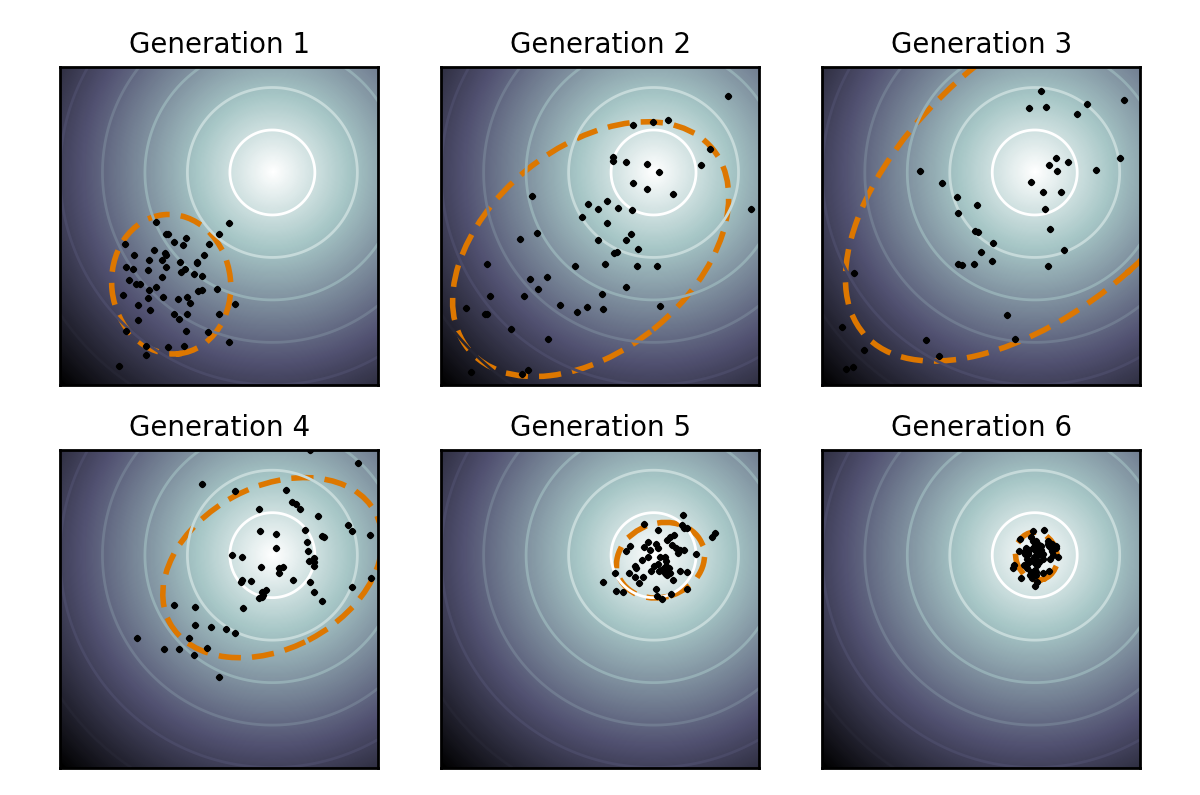
\includegraphics[width=7cm]{images/CMA_ES.png}
 \caption{\label{CMA-ES}Illustration of an actual optimization run with CMA-ES on a simple two-dimensional problem. The spherical optimization landscape is depicted with solid lines of equal-values. The population (dots) is much larger than necessary, but clearly shows how the distribution of the population (dotted line) changes during the optimization. \href{https://en.wikipedia.org/wiki/CMA-ES#/media/File:Concept_of_directional_optimization_in_CMA-ES_algorithm.png}{\color{blue}{Source}}}
 \label{CMA-ES}
\end{figure}

\bigbreak

\subsubsection{NEAT}
Since the architecture of a neural network (e.g. number of layers, size of each layer, recurrent units) can have a strong impact on final performance, this technique evolves both network structure and neuron weights on the final network. The NeuroEvolution of Augmenting Topologies algorithm (NEAT) created in 2002 (\cite{NEAT_1, NEAT_2}) presents solutions to 3 fundamental issues in the evolution of neural networks:

\begin{itemize}
    \item \textbf{Crossover between different structures}: NEAT provides a genotype-to-phenotype mapping based on mutations (Fig. \ref{NEAT}).
    \item \textbf{Protection of topological innovation}: The speciation mechanism evaluates candidates by comparing them to similar architectures to allow new structures to mature without being instantly eliminated. 
    \item \textbf{Minimization of structural complexity}: Nodes are added to a minimal initial structure in order to prevent networks from being too big without benefits.
\end{itemize}
\bigbreak

Multiple variants have been created from NEAT, including rtNEAT \cite{rtNEAT} for real-time neuroevolution, FS-NEAT \cite{FS-NEAT} for feature selection, or HyperNeat based on indirect encoding \cite{HyperNEAT}.

\begin{figure}[H]
 \centering
 \captionsetup{justification=centering, margin=0.5cm}
 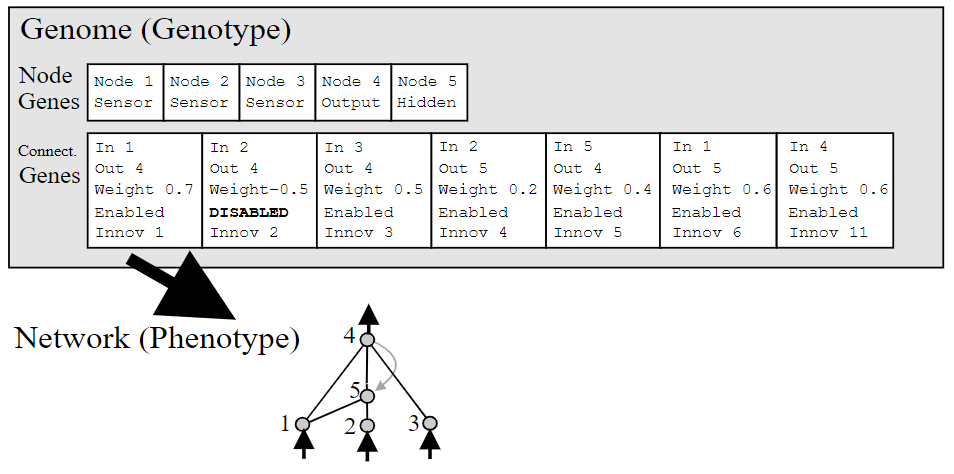
\includegraphics[width=7cm]{images/neat.png}
 \caption{\label{NEAT}NEAT genotype-to-phenotype mapping example. A genotype is depicted that produces the shown phenotype. There are 3 input nodes, one hidden, and one output node, and seven connection definitions, one of which is recurrent. \cite{NEAT_2}}
 \label{fig:NEAT}
\end{figure}


Evolve weight only: CMAES + NN
Evolve weight + structure: NEAT

\subsection{Indirect encoding}
Goal: reuse the same information multiple time, reduce the search space to a more efficient one
Principle: encode the weights of a NN with an evolved program

The second approach uses an intermediary program, optimized through an evolutionary algorithm, to generate the synaptic weights of the final neural network based on their positions. 

HyperNEAT \cite{HyperNEAT} uses a Compositional Pattern Producing Network (CPPN) \cite{CPPN} optimized through a NEAT-based process to create the final network. This allows the final network to be larger without increasing the size of the space to explore, since the same CPPN can be used on any number of neurons.

As Compositional Pattern Producing Networks implement multiple activation functions including Gaussian, sigmoid, and periodic functions, they can produce connectivity patterns with symmetries based on the positions of the neurons, better exploiting regularities in the task.

\section{Quality Diversity approaches}

\section{Coevolution}

%%% Local Variables: 
%%% mode: latex
%%% TeX-master: "isae-report-template"
%%% End: 
\chapter{Breezy Project: a DOTA 2 competition}
\label{chap:dota}

During the first month of my internship I teamed up with my supervisor \addlink{https://www.linkedin.com/in/dennis-g-wilson/}{Assoc. Prof. Dennis Wilson} and my fellow Research Intern \addlink{https://www.linkedin.com/in/lucashervier/}{Lucas Hervier} to participate in an Evolutionary Reinforcement Learning competition held as part of the international Genetic and Evolutionary Computation Conference, known as GECCO 2020, on the DOTA 2 video game. \\
The agents we submitted are available on \addlink{https://github.com/d9w/DotaBot}{GitHub}, and the source code has been \addlink{https://github.com/d9w/Project-Breezy-DOTA-Evolutionnary}{made open-source}.

\section{Context}
\subsection{Video games and Machine learning}
In 2018 the video game industry generated sales of more than US\$130 billion, reaching around 2 billion players around the world. Because video games can provide complex tasks necessitating short- and long-term planning in a controlled environment with no risks to humans \cite{Games_AI}, they also provide an excellent test-bed for Artificial Intelligence (AI) systems. Multiple learning agents have been tested on the Arcade Learning Environment based on Atari 2600 games \cite{Atari}, including Reinforcement Learning (RL) techniques like Deep Q Networks \cite{DQN} and Agent57 \cite{agent57}. Other games such as StarCraft, DOTA2, Mario, or Doom, have also been extensively used as machine learning benchmarks.

Since the reward in games is often sparse, making the learning signal weak, gradient-based methods might struggle for the optimization of neural network parameters. Evolutionary Strategies (ES), which estimate the gradient of the objective function without needing an explicit gradient definition, have been used to optimize Deep Convolutional Neural Networks \cite{CMAES_DL}, and the evolution of synaptic weights have been demonstrated to be competitive with deep RL methods\cite{deep_neuroevo}.\\

\subsection{OpenAI Five}
From 2016 to 2019, \addlink{https://openai.com/about/}{OpenAI} published work on the \addlink{https://openai.com/projects/five/}{OpenAI Five project}, an AI trained to play Dota 2 first in 1v1, and then extended to 5v5. OpenAI Five achieved a \addlink{https://arena.openai.com/#/results}{99.4\% win rate} against human players of any rank and \addlink{https://openai.com/blog/openai-five-defeats-dota-2-world-champions/}{defeated the world champions} twice in a live tournament, while also showing cooperation capabilities with humans. 

However, most of the technical details of the AIs trained for this project still remain unknown and unpublished, from the model architecture to the interface used to communicate with the game developed in partnership with Valve. Hence, further work and results reproduction are harder to implement, adding to the computational constraint (OpenAI Five required 764 petaflop/s-day operations for \textbf{over 10,000 years of games} against itself, totalling around $6.6.10^{22}$ operations). This makes the use of Dota 2 as a RL benchmark and its use in the development of open-source RL algorithms still an open problem. 

\subsection{Project Breezy}

In this context, \addlink{https://web.cs.dal.ca/~dota2/?page_id=353}{Project Breezy} is a competition created by Robert Smith and Malcolm Heywood from Dalhousie University to develop a DOTA 2-playing bot evolved with evolutionary algorithms, in a 1-versus-1 symmetrical match-up. 

For this purpose, they implemented and published a server interfacing with the Dota 2 game. As this work was not officially supported by Valve there may still be a performance difference compared to the system used to train openAI Five, but it provides an open-source tool for benchmarks.

We entered this competition as an opportunity to try and test neuroevolution algorithms on a complex real-time game, and as a step towards the development of a comprehensive benchmark of Evolutionary Reinforcement Learning algorithms as described in Chapter \ref{chap:berl}.

\section{DOTA 2 as a RL environment}
\subsection{The game}

Produced by Valve and available on its platform \addlink{https://store.steampowered.com/app/570/Dota_2/}{Steam}, \addlink{https://en.wikipedia.org/wiki/Dota_2}{Dota 2} is the sequel of Defense of the Ancients (DotA), a community-created game mod for Warcraft III that popularised the Multiplayer Online Battle in Arena (\addlink{https://en.wikipedia.org/wiki/Multiplayer_online_battle_arena}{MOBA}) video game genre. In Dota 2, 2 teams (called "Radiant" and "Dire") of 5 players compete to destroy the main structure of the enemy's base (the "Ancient") in a real-time strategy game, each player controlling one of the 119 possible characters (the "heroes").

\begin{figure}[H]
 \centering
 \captionsetup{justification=centering, margin=0.5cm}
 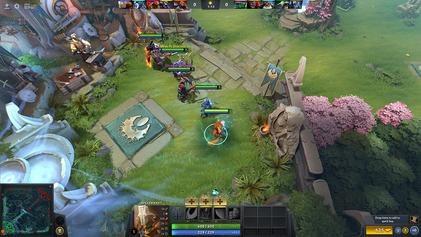
\includegraphics[width=8cm]{images/Dota_2_Gameplay_Aug_2017.jpg}
\caption{A game of Dota 2 in progress, showing the Radiant team inside their base at the beginning of a match}
 \small\textsuperscript{\url{https://en.wikipedia.org/wiki/Dota_2}}
 \label{fig:dota-2-game}
\end{figure}

The game takes place on a square map (cf fig. \ref{fig:dota-2-map}) which contains both team-controlled buildings (e.g. towers, barracks) that the other team can attack, and neutral objectives (e.g. Roshan). Team bases are situated in the bottom-left and top-right corners respectively, with 3 lanes joining them called the top (through the top-left corner), the middle (diagonally), and the bottom (through bottom-right corner) lane, each guarded by towers and around which most early gameplay happens. Creeps are basic AI-controlled units that periodically spawn for each team at the barracks and walk down the lane to help destroy enemy buildings. Dealing the last hit ("last hitting") an enemy creep is rewarded with money, which allows to buy items influencing the player's hero strengths. Last hitting a creep of the same team allows to deny them from the enemy. 

\begin{figure}[H]
 \centering
 \captionsetup{justification=centering, margin=0.5cm}
 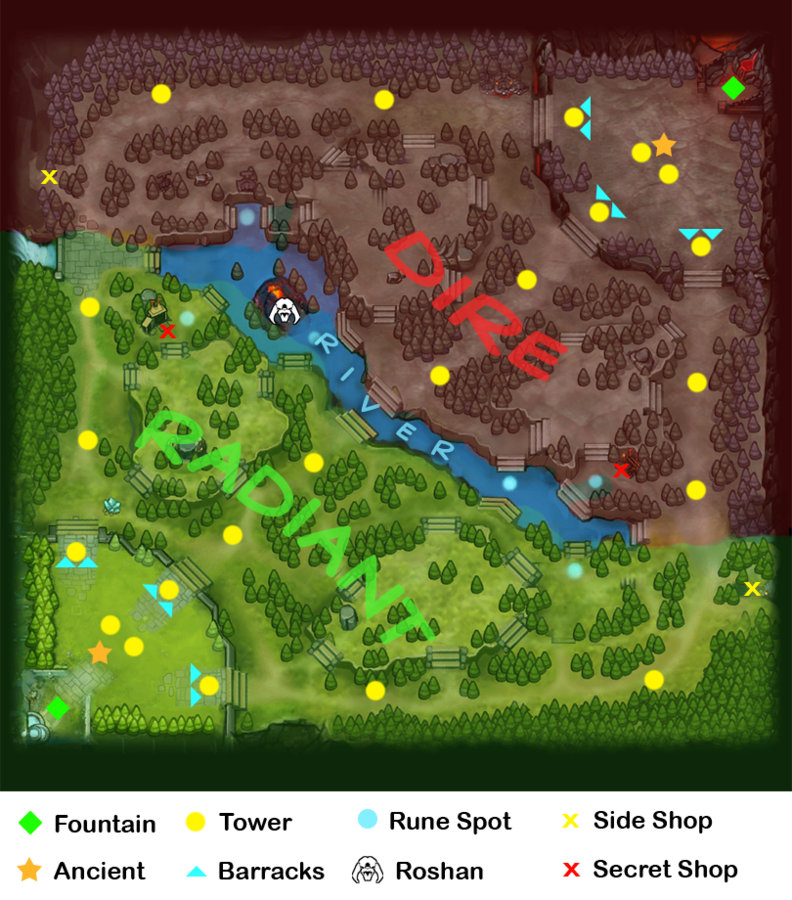
\includegraphics[width=8cm]{images/dota-map.png}
\caption{Labelled Dota 2 map as of version 7.20}
 \small\textsuperscript{\url{https://dota2.gamepedia.com/Map}}
 \label{fig:dota-2-map}
\end{figure}

The 1v1 game mode opposes only 1 player in each team, and can be won by either killing the enemy twice, or destroying the first enemy tower on the middle lane. \\
The game mode used for this competition additionally fixes the heroes to be \addlink{https://dota2.gamepedia.com/Shadow_Fiend}{Shadow Fiend} for both players, for balancing purposes.

\subsection{Project Breezy Software}
\addlink{https://web.cs.dal.ca/~dota2/?page_id=353}{Project Breezy} provides software to enable communication with the Dota 2 game by opening a server communicating with the game instance. The agent, through a Python server, interacts with the Breezy server, getting the game state and sending action orders. The game state contains 310 features such as health points, hero position, creeps positions, or spell cooldowns. 29 actions are available, including movementS, spell casting, or attacking.

We noticed the server actually returned the state before effectuating an action, adding a delay in the information processing. Even though evolved models might still work thanks to internal memory, recurrence, or implicit prediction, this made predicting the next state in the simulator and analyzing behaviors significantly harder. 

\subsection{Challenges}
\begin{minipage}{\linewidth}
Evolving Neural Networks to play Dota 2 is subject to multiple constraints:
\begin{itemize}
    \item \textbf{Processing time}: Since DOTA 2 is a real-time game, the generated neural networks needs to be fast to evaluate at each step.
    \item \textbf{Evaluation time}: Even sped up, evaluating a policy requires running a full game in a simulator, hence the number of evaluations is a strong limiting factor.
    \item \textbf{Network size}: Due to the large size of the game state provided by the Breezy server and the hight number of possible actions, generated neural networks might require large architectures, hence increasing computation time and problem dimensionality.
    \item\textbf{Network complexity}: Since Dota 2 requires both short- and long-term planning, more complex architectures might be required 
    \item \textbf{Fitness sparsity}: Since the fitness used rewards dealing damage and last hitting, many behaviors that do not get close enough to the enemy have the same fitness, hence information about the quality of an individual is rare and requires already advanced policies
\end{itemize}
\end{minipage}

\section{Our approach}

\subsection{Problem Modeling}
\label{sec:representation choice}

\subsubsection{Fitness Function}
As in order to win a 1v1 a player needs to either kill the opponent twice or to take his first mid tower, we took into account the number of times we killed the opponent champion and the opponent tower health in the individual evaluation. Moreover, to succeed in one of those two tasks one would also need good laning skills, so we also added the amount of gold collected (\textit{net worth}), the number of last hits, and the number of denies. We also punished being killed and behaviors causing an early stopping as referenced in section \ref{sub:early-stop}.

\begin{minipage}{\linewidth}
The final fitness function is hence as follows:

\begin{equation*}
\label{eq:fitness}
\begin{minipage}{0.7\textwidth}
% \begin{multline*}
\begin{split}
 fitness & = netWorth + 100*lastHits + 100*denies\\
         & + 2000*ratioTowerHealth + 1000*nbKill\\
         & - 250*nbDeath - 500*earlyStop\\
 \end{split}
% \end{multline*}
\end{minipage}
\end{equation*}
\end{minipage}


\subsubsection{Behavior Space}
Our goal with a Quality-Diversity approach was to observe individuals with highly diverse behaviors to increase our chances of finding interesting ones. Therefore, we needed a characterization of the behavior space to differenciate playstyles. 
We described the behavior in a discretized 2-dimensional space featuring the \textit{total damage made to the opponent champion} and the \textit{percentage of the opponent tower health taken} as axes, since the objective was either to kill the opponent champion or to take his tower. 

\subsection{Reducing the evaluation cost}
We quickly realized that one of the main difficulty of this challenge was to deal with the evaluation cost of the fitness. Indeed, in order to evaluate an agent we need him to play a full DOTA2 game which can take up to several minutes in real time, even with a tenfold speeding. Since Evolutionnary Algorithms (EAs) require a large number of function evaluations, we had to find a way to cope with this issue. 

\subsubsection{Early stopping}
\label{sub:early-stop}
A simple but efficient way of reducing the evaluation time was to use an Early Stopping mechanism. We decided to stop the evaluation of an agent if he did not kill a creep after 5min of DOTA time. This functionality reduced the time loss due to static individual, and the evaluation length of "coward individuals" avoiding fights.

\subsubsection{Neural-base simulator}
Since an evaluation is time consuming, I developped a \addlink{https://github.com/TemplierPaul/Dota_Simulator}{\textbf{Dota Simulator}} to predict game state evolutions from previous state and chosen action, using a neural network trained on more than 100 games played with a random policy.

The  main part of the simulator was implemented in object-orient Python to process game data, remove constant features to reduce the size of the network, create and train the neural network, and act as a simulator with a Gym-like API. A Julia wrapper was then added, to allow plugging the simulator into the rest of the project.\\
Jupyter notebooks were also used to explore data and train the networks on the \addlink{https://research.google.com/colaboratory/local-runtimes.html?hl=en}{Google Colaboratory} platform.  

3 networks of growing depths based on the UNet \cite{unet} architecture, and simple feed-forward neural networks were tried, with no particular performance difference observed. Finally, a feed-forward network with few layers of many neurons was chosen.  

\begin{figure}[H]
 \centering
 \captionsetup{justification=centering, margin=0.5cm}
 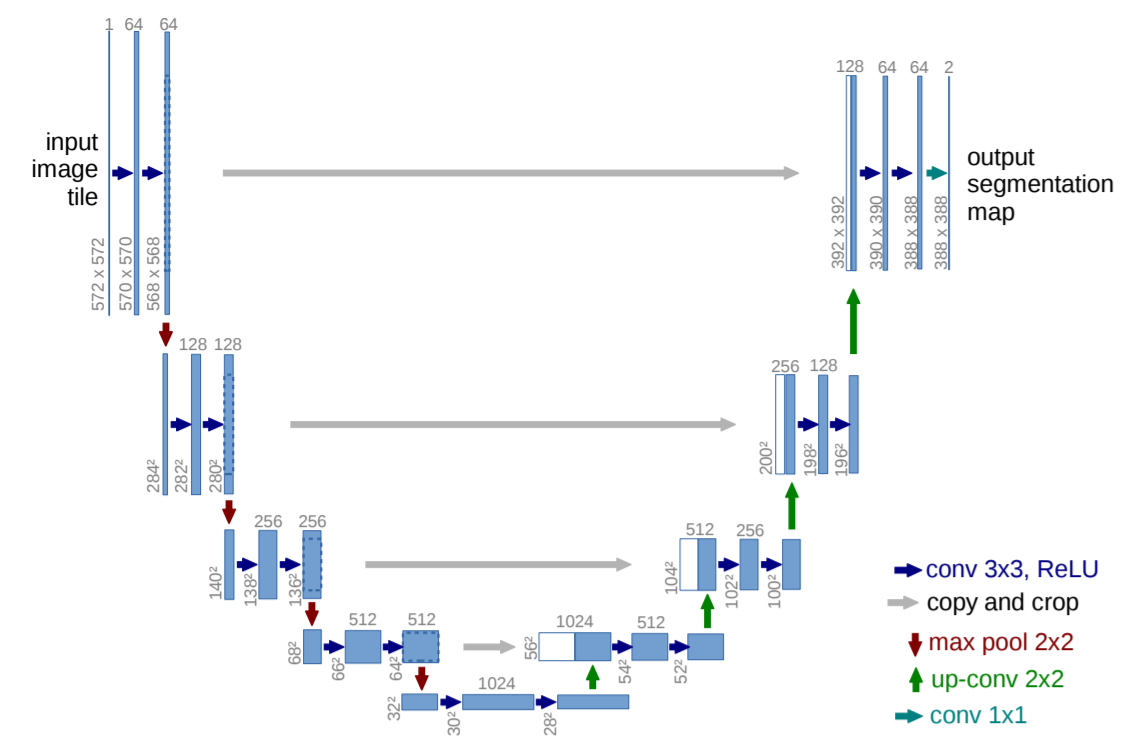
\includegraphics[width=8cm]{images/unet.PNG}
\caption{Example U-net architecture in \cite{unet}, each blue box corresponding to a multi-channel feature map.}
 \label{fig:dota-2-map}
\end{figure}

The simulator was used in the offsprings generation phase to encourage diversity:
\begin{itemize}
    \item offsprings are generated for 10 times the size of population 
    \item 100 game steps are simulated for each offspring, and the actions taken at each step are stored
    \item the actions taken by each individual are used to select the \textit{population size} most unique offsprings based on behavior
    \item those individuals are added to the new population and evaluated in the real game to compute the real fitness
\end{itemize}

By doing so we are seeing much more mutation and/or crossover. Moreover, taking the individuals the more distant from each other increases our chances to cover the behavior space.

\subsection{Algorithms}
We chose to train both CGP Individuals  \cite{CGP} and NEAT Individuals \cite{NEAT_1}, as defined in the respective papers, in a MAP-Elites algorithm. They were implemented with \href{https://github.com/d9w/CartesianGeneticProgramming.jl}{\textbf{CartesianGeneticProgramming.jl}} for the CGP agent, and a custom NEAT agent developed at \href{https://github.com/d9w/NEAT.jl}{\textbf{NEAT.jl}} for this challenge.

As we believed the best way to find interesting individuals, either with NEAT or with CGP, was to explore the behavorial space, we based the exploration on the \textbf{Illuminating search spaces by mapping elites} \cite{MapElites} work, implementing a MAP-Elites method to find policies of varying styles, focusing more on killing the enemy, on destroying the tower, or balancing both. 
As the evaluation of a policy relies on a full game which can be heavily influenced by small perturbations, including time delays due to the Breezy software communication method, the behavior space can be seen as a noisy domain. Hence, we believe using the work of \cite{noisy-map-elites} on MAP-Elites in noisy domains using deep grids to consider this property and  make the evaluation more reliable could improve future work, since it was published too late for us to implement it. 

\section{Results}

Results were announced at GECCO 2020 on July 12\textsuperscript{th} by the organizers. \\
9 teams had registered to the competition, but only 2 -including us- provided code to be evaluated, among which we ranked first. \\

\begin{figure}[H]
\centering
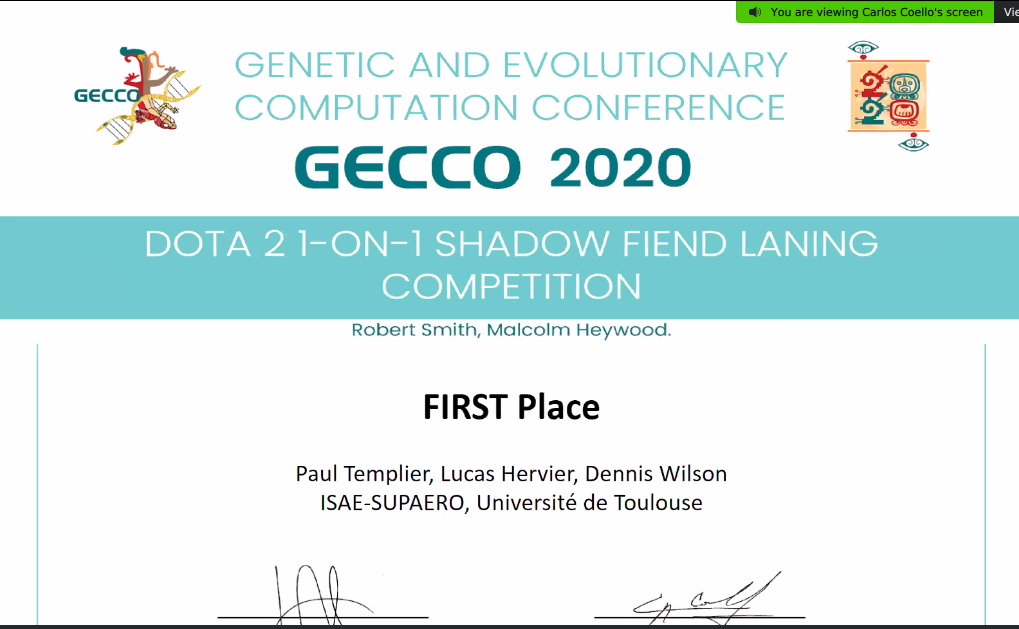
\includegraphics[width=12cm]{images/breezy-win.png}
\caption{Competition results announcement at GECCO 2020}
\end{figure}

%%% Local Variables: 
%%% mode: latex
%%% TeX-master: "isae-report-template"
%%% End: 
\chapter{BERL.jl for RL benchmarking}
\label{sec:berl}

\section{Motivation and structure}

\section{Benchmark tasks}
\subsection{Atari}

\subsection{Gym and PyBullet}

\section{Algorithms whishlist}
\subsection{CGP}
\subsection{Neuroevolution algorithms}
Needed a Julia implementation => NeuroEvolution.jl

%%% Local Variables: 
%%% mode: latex
%%% TeX-master: "isae-report-template"
%%% End: 
\chapter{Developping NeuroEvolution.jl}
\label{chap:neuroevo}

\href{https://github.com/TemplierPaul/NeuroEvolution.jl}{\color{blue}{NeuroEvolution.jl}} is a Julia library I developed to implement multiple neuroevolution algorithms for BERL. It includes \textbf{NEAT} (NEuroEvolution of Augmenting Topologies) and \textbf{HyperNEAT} Hypercube-based NEAT), and an implementation of a direct weights optimization in a fix network using \textbf{CMAES} (Covariance matrix adaptation evolution strategy) is in progress to complete it. 

The concepts powering the NEAT algorithm may seem relatively simple and clear as described in the literature, making it a quite elegant solution. \\
However, its implementation raises multiple complex issues, turning out to be rather intricate. The obstacles met when implementing part of it for an earlier \href{https://github.com/TemplierPaul/Genepy}{\color{blue}{personal project}},  and in the \href{https://github.com/d9w/NEAT.jl/tree/master/src}{\color{blue}{NEAT agent}} developed for the Breezy competition (cf chapter \ref{chap:dota}), helped design a more reliable structure and drastically reduced the development time.

This chapter aims at presenting the choices made during the design and development of NeuroEvolution.jl, its architecture and the main principles ruling it. 

\section{NEAT implementation}
I developed the NEAT algorithm based on the original papers \cite{NEAT_1} and \cite{NEAT_2}, taking into account the remarks and indications of the author on \href{https://www.cs.ucf.edu/~kstanley/neat.html#FAQ2}{
\color{blue}{his website}}. \\
The \href{https://github.com/FernandoTorres/NEAT}{\color{blue}{reorganized version}} of the original C++ implementation of NEAT also provided insight into the algorithm, although some parts were approached differently, taking the papers as reference.

\subsection{NEAT Individual}

Based on Cambrian.jl, NeuroEvolution.jl uses an abstract type \code{NEATIndiv} from which the structure \code{NEATIndividual} inherits. This allows to build new NEAT-like individuals using the same methods with additional features, like HyperNEAT which relies on the NEAT algorithm for evolution, but integrates a different evaluation procedure. \code{NEATIndiv} inherits from \code{Cambrian.Individual} to use Cambrian's architecture.

A \code{NEATIndividual} object contains a dictionary mapping an innovation number to a gene, which represents a connection between two neurons, a list of neurons defined by their positions, a dictionary mapping each neuron position to the activation function of the corresponding neuron, a \code{Network} object containing the neural network built from the genome, and a list of the fitness of the individual as required by Cambrian.

\begin{minipage}{\linewidth}
\begin{lstlisting}[language=Julia, caption=NEAT Individual (\href{https://github.com/TemplierPaul/NeuroEvolution.jl/blob/master/src/individual.jl}{\color{blue}{Source}})]
abstract type NEATIndiv <: Cambrian.Individual end

mutable struct NEATIndividual <: NEATIndiv
    genes::Dict
    fitness::Array{Float64}
    neuron_pos::Array{Float64}
    network::Network
    activ_functions::Dict
end
\end{lstlisting}
\end{minipage}

\subsection{Neuron position and Execution order}
\label{subsec:NEAT_neur_pos}

On of the main issues encountered when implementing NEAT in previous personal projects is the order of computation of the neurons. Due to the way it grows, the NEAT network can build recurrent connections, including bidirectional relationships with one connection from neuron A to neuron B, and one connection from B to A. Then, propagating depth from the output neurons to make sure all previous neuron values have been computed leads to an infinite loop between A and B, each one needing to be computed before the other. 

To prevent that issue and reduce the time needed to build the network, this implementation of NEAT was inspired by the work of \cite{wilson2018positionalcgp} in which the position of a CGP node is described as a floating point value. The execution order is then available by design since they can be executed sequentially based on their positions. Recurrent connections are defined by destination neurons being before origins, which makes possible to allow or block them easily at mutation. 

This representation also removes the propagation time concept, making the NEAT network closer to standard neural networks. 

The position of a neuron is defined as follows:
\begin{itemize}
    \item All input neurons are placed with negative integer positions.  
    \item The bias neuron (constant equal to 1) is placed at $0$.  
    \item All output neurons are placed at positive integer positions, starting at $1$.
    \item All other neurons are placed with positions in $]0, 1[$.
\end{itemize}

\begin{figure}[H]
\centering
\captionsetup{justification=centering,margin=2cm}
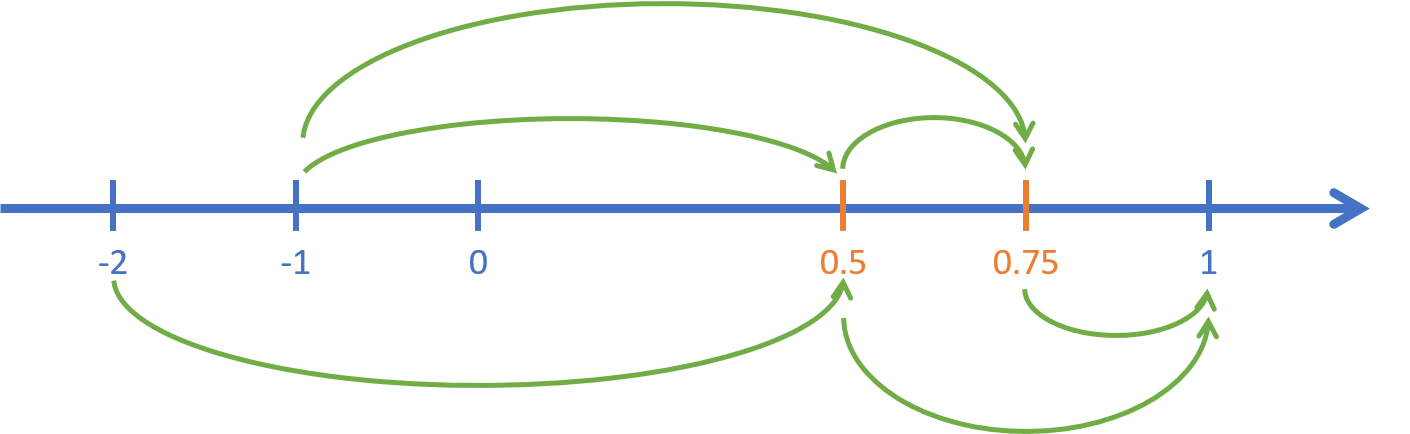
\includegraphics[width=10cm]{images/NEAT_position.png}
\caption{Example of NEAT individual as neurons defined by position and feed-forward connections, with 2 input features, 1 output neuron and 2 hidden neurons.}
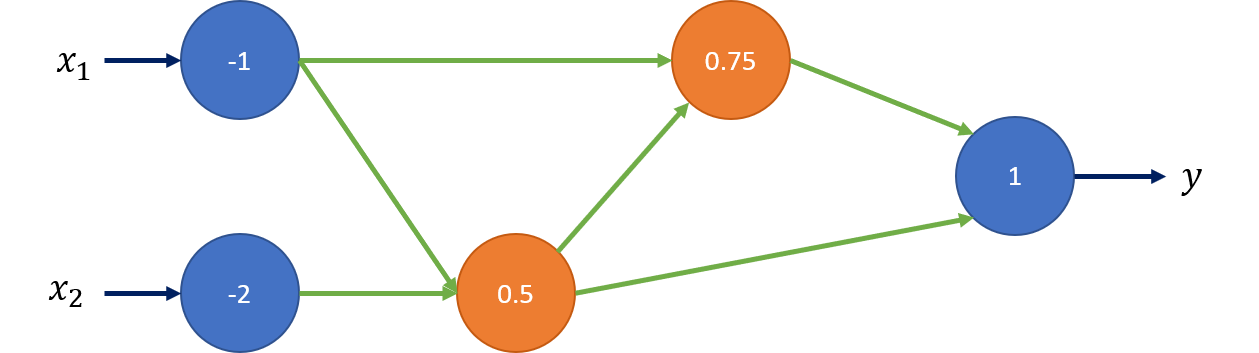
\includegraphics[width=10cm]{images/NEAT_network.png}
\caption{Neural Network generated from the above individual.}
 \label{NEAT_network}
\end{figure}

Neurons added through mutation of a connection are placed at a random position between the origin node of the connection at $p_o$ and the destination node at $p_d$, so that the order of execution is not modified. \\
The position of the new neuron is therefore randomly drawn in $]p_o, p_d[ \: \cap \: ]0, 1[$.

Because of this structure, and to avoid edge cases, connections between 2 output neurons are forbidden. Connections towards input and bias neurons are blocked too, since their values are fixed to the input vector and to 1 respectively.

When computing the network's output, its neurons are sorted by ascending position. Since the position determines the neuron type, choosing the update type is simple:

\begin{minipage}{\linewidth}
\begin{lstlisting}[language=Julia, caption=NEAT network processing (\href{https://github.com/TemplierPaul/NeuroEvolution.jl/blob/master/src/process.jl}{\color{blue}{Source}})]
for p in indiv.neuron_pos
    if p < 0 # Input neurons
        indiv.network.neurons[p].output = 
                    last_features[Int(-p)]
    elseif p == 0 # Bias neuron
        indiv.network.neurons[p].output = 1
    else # Hidden and output neurons
        compute!(indiv.network.neurons[p], 
                    indiv.network.neurons)
    end
end
\end{lstlisting}
\end{minipage}

\subsection{Run configuration}

The parameters to run NEAT are defined in a \href{https://github.com/TemplierPaul/NeuroEvolution.jl/blob/master/cfg/test.yaml}{\color{blue}{YAML file}}  that is read at runtime. It includes:

\begin{itemize}
    \item Cambrian settings: population size, number of generations
    \item Input and output size of the network
    \item Speciation parameters
    \item Mutation probabilities for each mutation type
    \item Available activation functions including sigmoid, trigonometric functions, absolute value, identity, or ReLU. 
\end{itemize}

One of the available activation functions is randomly selected when a new neuron is created, allowing the implementation of a Compositional Pattern-Producing Network (CPPN) by making multiple ones available. The default activation function for NEAT is the sigmoid. 

\subsection{Crossover and innovation number}
A usually delicate part of the implementation of NEAT lies in the management of the innovation number, which tracks genes across the population and guarantees the same gene is recognized on both sides during crossover.

In this implementation, and according to Cambrian's structure, a configuration dictionary is passed across the algorithm to each method requiring run parameters, built from the YAML configuration file. The innovation number is stored inside and updated after each mutation adding a gene. 

Using a dictionary in the individual to store each gene linked to its innovation number allows to compare genomes more efficiently at crossover than an array of genes. 

\subsection{Speciation threshold}
NEAT relies on speciation to update its population:
\begin{itemize}
    \item If individuals are closer than the speciation threshold, they get put in the same species
    \item The fitness of each individual is computed with explicit fitness sharing, hence divided by the size of the population of their species
    \item Offspring are distributed among species depending on the mean (or the max) fitness in the current members of the species
    \item Reproduction is computed in each species by selecting parents randomly in the top members of the species (or based on their individual fitness in a tournament selection) and applying either mutation or crossover.
    \item All offspring are assigned to the closest species
\end{itemize}

However as generations occur the distance between genomes grows and the algorithm tends to assign a different species to each individual, hence causing hundreds of species to appear. In order to keep a stable number of species, K.O.Stanley introduces on his website a changing threshold, increasing of decreasing by a fix amount in order to keep the number of active species stable. 

I introduced a slightly modified version of this algorithm as \code{update\_threshold!}, which modifies the threshold by an amount scaled on the ratio: $$current\_species\_number \over wanted\_species\_number$$

This solution yields a very stable number of species, although usually higher than the wanted number.

\subsection{NEAT in a standard Genetic Algorithm}

The goal of using Cambrian as a framework in this implementation also was to allow for a high compatibility with other algorithm so that the coding blocks defined for NEAT could be reused in classical evolutionary algorithms, from a Genetic Algorithm (GA) to a Quality-Diversity method as envisioned in the Breezy competition (cf chapter \ref{chap:dota}). 

Hence, I finally implemented a simple wrapper to use the NEAT Individual and its mutation and crossover operators in a standard Genetic Algorithm, ignoring the specific species-based populate function for the standard Cambrian \code{ga\_populate} function.

\begin{minipage}{\linewidth}
\begin{lstlisting}[language=Julia, caption=Genetic Algorithm populate for NEAT  (\href{https://github.com/TemplierPaul/NeuroEvolution.jl/blob/master/src/evolution.jl}{\color{blue}{Source}})]
function neat_ga_populate!(e::Evolution)
    mut::Function=i::NEATIndiv -> 
                    NeuroEvolution.mutate(i, e.cfg)
    cross::Function=(p1, p2) -> 
                    NeuroEvolution.crossover(p1, p2, e.cfg)
    Cambrian.ga_populate!(e, mutation=mut, crossover=cross)
end
\end{lstlisting}
\end{minipage}

This compatibility with other Cambrian algorithms allows to easily use the NEAT individual in other settings such as Quality-Diversity methods or open-ended evolution, thus helping in new algorithms research.

\section{Adding HyperNEAT}
HyperNEAT \cite{HyperNEAT} introduces indirect encoding by using a CPPN (Compositional Pattern-Producing Network \cite{CPPN}) to determine the weights of a neural network with a fix architecture. Since the CPPN can be evolved with the NEAT algorithm for HyperNEAT, most evolutionary methods in NeuroEvolution.jl can be reused. \\ 
However, instead of evaluating the evolved network (the CPPN) to solve the problem, the CPPN is used to determine the weights of a network with fixed architecture, referenced here as the \code{final network}. 

\subsection{HyperNEAT Individual}

HyperNEAT was added to NeuroEvolution.jl by creating a structure \code{HyperNEATIndiv}, inheriting from \code{NEATIndividual} like \code{NEATIndiv}. Thus, functions affecting the evolved network (e.g. mutation, crossover, populate) take as arguments any object inheriting from the abstract type \code{NEATIndividual}, and are blind to whether NEAT or HyperNEAT is used. Conversely, other functions related to the evaluation of an individual (e.g. evaluate, build, process) are algorithm-specific and are defined for each individual type.

\begin{minipage}{\linewidth}
\begin{lstlisting}[language=Julia, caption=HyperNEAT Individual (\href{https://github.com/TemplierPaul/NeuroEvolution.jl/blob/master/src/HyperNEAT.jl}{\color{blue}{Source}})]
mutable struct HyperNEATIndividual <: NEATIndiv
    genes::Dict
    fitness::Array{Float64}
    neuron_pos::Array{Float64}
    network::Network
    activ_functions::Dict
    hn_net::GridNetwork
end
\end{lstlisting}
\end{minipage}

\code{HyperNEATIndividual} uses the same structure as \code{NEATIndividual}, adding a \code{hn\_network} field to store the generated final network described in subsection \ref{sub:final-hn-net}.

\subsection{Final network definition}
\label{sub:final-hn-net}
The final network is a feed-forward, fully-connected neural network with a fixed architecture. It is build from an array of \code{Layer} objects, each containing the output values of a neurons layer, and an array of \code{Connection} objects linking 2 layers and implementing weights. 

\begin{minipage}{\linewidth}
\begin{lstlisting}[language=Julia, caption=HyperNEAT final network (\href{https://github.com/TemplierPaul/NeuroEvolution.jl/blob/master/src/HyperNEAT.jl}{\color{blue}{Source}})]
mutable struct GridNetwork
    layers::Array{Layer}
    connections::Array{Connection}
end
\end{lstlisting}
\end{minipage}

The \code{build!} method creates the final network and sets its weighs with the CPPN, while the \code{process!} method computes the output of the final network. This approach allows to only build the network once, but increases complexity by adding a step to place between mutation and evaluation.

\subsection{Run configuration}

Using HyperNEAT requires a \href{https://github.com/TemplierPaul/NeuroEvolution.jl/blob/master/cfg/hyperneat.yaml}{\color{blue}{specific YAML file}} which adds information about hidden layers and structure of the generated network to the standard NEAT parameters. 

Although the default architecture for the final networks only links a layer of neurons to the previous one, toggling the \code{hn\_link\_all\_layers} parameter to \code{true} creates a connection between each layer and all the previous ones, for a more complex architecture. Using a CPPN for weights generation makes it possible to use such architecture without expanding the search space, contrary to direct encoding. 

\section{CMA-ES applied to neuroevolution}

%%% Local Variables: 
%%% mode: latex
%%% TeX-master: "isae-report-template"
%%% End: 
\chapter{Results}
\label{sec:results}

\section{Comparison setup}
\subsection{Algorithms and parameters}

\subsection{Environments}

\section{Analysis}

\subsection{Performance}
Max fitness
\begin{figure}[H]
\centering

\includegraphics[width=8cm]{images/data_meme.jpg}
\caption{Placeholder}
\end{figure}
      
      
\subsection{Efficiency}
Number of evaluations to reach the same fitness
\begin{figure}[H]
\centering
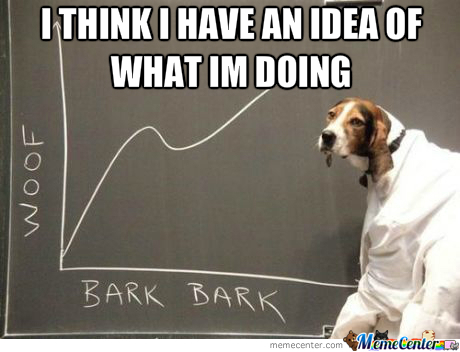
\includegraphics[width=8cm]{images/data_meme2.jpg}
\caption{Placeholder}
\end{figure}

%%% Local Variables: 
%%% mode: latex
%%% TeX-master: "isae-report-template"
%%% End: 
\chapter*{Conclusion}
\addcontentsline{toc}{chapter}{Conclusion}
\markboth{Conclusion}{Conclusion}
\label{chap:conclusion}
%\minitoc


Lorem ipsum dolor sit amet, consectetur adipiscing elit. Sed non risus. Suspendisse lectus tortor, dignissim sit amet, adipiscing nec, ultricies sed, dolor. Cras elementum ultrices diam. Maecenas ligula massa, varius a, semper congue, euismod non, mi. Proin porttitor, orci nec nonummy molestie, enim est eleifend mi, non fermentum diam nisl sit amet erat. Duis semper. Duis arcu massa, scelerisque vitae, consequat in, pretium a, enim. Pellentesque congue. Ut in risus volutpat libero pharetra tempor. Cras vestibulum bibendum augue. Praesent egestas leo in pede. Praesent blandit odio eu enim. Pellentesque sed dui ut augue blandit sodales. Vestibulum ante ipsum primis in faucibus orci luctus et ultrices posuere cubilia Curae; Aliquam nibh. Mauris ac mauris sed pede pellentesque fermentum. Maecenas adipiscing ante non diam sodales hendrerit. Ut velit mauris, egestas sed, gravida nec, ornare ut, mi. Aenean ut orci vel massa suscipit pulvinar. Nulla sollicitudin. Fusce varius, ligula non tempus aliquam, nunc turpis ullamcorper nibh, in tempus sapien eros vitae ligula. Pellentesque rhoncus nunc et augue. Integer id felis. Curabitur aliquet pellentesque diam. Integer quis metus vitae elit lobortis egestas. Lorem ipsum dolor sit amet, consectetuer adipiscing elit. Morbi vel erat non mauris convallis vehicula. Nulla et sapien. Integer tortor tellus, aliquam faucibus, convallis id, congue eu, quam. Mauris ullamcorper felis vitae erat. Proin feugiat, augue non elementum posuere, metus purus iaculis lectus, et tristique ligula justo vitae magna. Aliquam convallis sollicitudin purus. Praesent aliquam, enim at fermentum mollis, ligula massa adipiscing nisl, ac euismod nibh nisl eu lectus. Fusce vulputate sem at sapien. Vivamus leo. Aliquam euismod libero eu enim. Nulla nec felis sed leo placerat imperdiet. Aenean suscipit nulla in justo. Suspendisse cursus rutrum augue. Nulla tincidunt tincidunt mi. Curabitur iaculis, lorem vel rhoncus faucibus, felis magna fermentum augue, et ultricies lacus lorem varius purus. Curabitur eu amet.

Lorem ipsum dolor sit amet, consectetur adipiscing elit. Sed non risus. Suspendisse lectus tortor, dignissim sit amet, adipiscing nec, ultricies sed, dolor. Cras elementum ultrices diam. Maecenas ligula massa, varius a, semper congue, euismod non, mi. Proin porttitor, orci nec nonummy molestie, enim est eleifend mi, non fermentum diam nisl sit amet erat. Duis semper. Duis arcu massa, scelerisque vitae, consequat in, pretium a, enim. Pellentesque congue. Ut in risus volutpat libero pharetra tempor. Cras vestibulum bibendum augue. Praesent egestas leo in pede. Praesent blandit odio eu enim. Pellentesque sed dui ut augue blandit sodales. Vestibulum ante ipsum primis in faucibus orci luctus et ultrices posuere cubilia Curae; Aliquam nibh. Mauris ac mauris sed pede pellentesque fermentum. Maecenas adipiscing ante non diam sodales hendrerit. Ut velit mauris, egestas sed, gravida nec, ornare ut, mi. Aenean ut orci vel massa suscipit pulvinar. Nulla sollicitudin. Fusce varius, ligula non tempus aliquam, nunc turpis ullamcorper nibh, in tempus sapien eros vitae ligula. Pellentesque rhoncus nunc et augue. Integer id felis. Curabitur aliquet pellentesque diam. Integer quis metus vitae elit lobortis egestas. Lorem ipsum dolor sit amet, consectetuer adipiscing elit. Morbi vel erat non mauris convallis vehicula. Nulla et sapien. Integer tortor tellus, aliquam faucibus, convallis id, congue eu, quam. Mauris ullamcorper felis vitae erat. Proin feugiat, augue non elementum posuere, metus purus iaculis lectus, et tristique ligula justo vitae magna. Aliquam convallis sollicitudin purus. Praesent aliquam, enim at fermentum mollis, ligula massa adipiscing nisl, ac euismod nibh nisl eu lectus. Fusce vulputate sem at sapien. Vivamus leo. Aliquam euismod libero eu enim. Nulla nec felis sed leo placerat imperdiet. Aenean suscipit nulla in justo. Suspendisse cursus rutrum augue. Nulla tincidunt tincidunt mi. Curabitur iaculis, lorem vel rhoncus faucibus, felis magna fermentum augue, et ultricies lacus lorem varius purus. Curabitur eu amet.

%%% Local Variables: 
%%% mode: latex
%%% TeX-master: "isae-report-template"
%%% End: 


\appendix

\bibliographystyle{authoryear-fr}
\bibliography{references}



\end{document}